\documentclass[%
reprint,
superscriptaddress,
% groupedaddress,
% unsortedaddress,
% runinaddress,
% frontmatterverbose,
% preprint,
% preprintnumbers,
% nofootinbib,
% nobibnotes,
bibnotes,
amsmath,
amssymb,
aps,
showkeys,
% pra,
prb,
% rmp, prstab, prstper, floatfix,
]{revtex4-1}

\usepackage{braket}
\usepackage{graphicx}
\graphicspath{{images_inkscape/}}
\usepackage{dcolumn}                    % Align table columns on decimal point
\usepackage{bm}                         % bold mathb
\usepackage{hyperref}                   % add hypertext capabilities
\usepackage[mathlines]{lineno}          % Enable numbering of text and display math
% \linenumbers\relax                    % Commence numbering lines

% \usepackage[showframe,%Uncomment any one of the following lines to test
% scale=0.7, marginratio={1:1, 2:3}, ignoreall,% default settings
% text={7in,10in},centering,
% margin=1.5in,      total={6.5in,8.75in},      top=1.2in,      left=0.9in,      includefoot,
% height=10in,a5paper,hmargin={3cm,0.8in},
% ]{geometry}

\newcommand{\iunit}[2]{\ensuremath{#1\,\text{#2}}}
\newcommand{\iket}[1]{\ensuremath{\Ket{#1}}}
\newcommand{\ibra}[1]{\ensuremath{\Bra{#1}}}
\newcommand{\ira}{\ensuremath{\,\rightarrow\,}}
\newcommand{\iRa}{\ensuremath{\qquad\Rightarrow\qquad}}
\newcommand{\ilra}{\ensuremath{\,\leftrightarrow\,}}
\newcommand{\iabs}[1]{\ensuremath{\left|#1\right|}}
\newcommand{\iabsSquared}[1]{\ensuremath{\left|#1\right|^2}}
\newcommand{\iratext}[1]{\ensuremath{\,\xrightarrow{\text{#1}}\,}}

\begin{document}

% \preprint{APS/123-QED}

\title{The superconducting twin qubit}
% \thanks{A footnote to the article title}%

\author{I.  V.  Antonov}  \affiliation{Royal Holloway, University of London,  Egham, TW20 0EX,
  UK} \affiliation{National Physical Laboratory, Hampton Road Teddington, TW11 0LW, UK}

\author{R. S.  Shaikhaidarov} \affiliation{Royal Holloway,  University of London,  Egham, TW20
  0EX, UK}

\author{V.  N.  Antonov} \affiliation{Skolkovo Institute of Science and Technology, Nobel str.
  3, Moscow,  143026, Russia} \affiliation{Royal  Holloway, University of London,  Egham, TW20
  0EX,  UK} \affiliation{Moscow  Institute of  Physics and  Technology, 29  Institutskiy per.,
  141700 Dolgoprudny, Moscow Region, Russia}

\author{O.V.  Astafiev} \affiliation{Skolkovo Institute of  Science and Technology, Nobel str.
  3, Moscow,  143026, Russia} \affiliation{Royal  Holloway, University of London,  Egham, TW20
  0EX, UK} \affiliation{National Physical Laboratory, Hampton Road Teddington, TW11 0LW, UK}

\date{\today}% It is always \today, today,
% but any date may be explicitly specified

\begin{abstract}
  In this work  we study a modification of  a flux qubit geometry --  a combination of
  two loops joined by a common Josephson  junction which will be called `twin-qubit'.  At the degeneracy flux-bias point, $ \Phi_0/2 $ in both loops, our twin qubit has energy
  spectrum plateaus and anharmonicity, more than 2 GHz. This flatness makes the qubit insensitive to
  a global  low-frequency flux  noise.  The  qubit is capacitively  coupled to  a transmission
  line, which  allows to experimentally  study it's  spectrum.
  We simulate the qubit and extract it's parameters with a standard quantum circuit model and compare the simulations with the experimental results.
\end{abstract}

\keywords{Flux-qubit}

\maketitle

%% Background
Superconducting  qubits  are  among  the most  promising  platforms  for  quantum  computing
technology. Typical  qubits are  on-chip aluminum structures  with Josephson  junctions (JJs),
whose geometry  can be  designed to  select an  operating energy,  state transition  rates and
sensitivity required in a particular environment.  Over  the past decade they have carried out
the   functionality   of   a   transistor   \cite{Astafiev_2010,   Hoi_2011,   Abdumalikov_2010,
  Astafiev_2010_2},  where a  control field  was used  to pass or block a  probe field  at a
different  frequency,  multiplexer  \cite{H_nigl_Decrinis_2018},  two  input signals  can  be  mixed  to
controllably generate a single output signal, and serial bus \cite{Shen_2005}.  Superconducting
qubits can  be fabricated using  standard nanofabrication  techniques and integrated  at scale
into quantum circuits \cite{Johnson_2010}.

One  of the  inherent limitations,  which  is encountered with superconducting qubits, is  a coherence  time,
$\tau_{\text{dec}}$, beyond  which quantum information  becomes lost. Two main sources of de-coherence are charge and flux fluctuations in vicinity of the qubit. Charge fluctuations are particular harmful for the qubits, where the charging energy, $E_C$, is large. In  flux qubit
architectures the JJ  energy $E_J$ dominates over  the charging energy  ($E_J/E_C \gg 1$),
which lowers  the device's  charge sensitivity  \cite{Orlando_1999,Chiorescu_2003,Mooij_1999}. Therefore a
family  of flux qubit designs  have led to  improvement of the coherence  times: shunted
flux qubit \cite{Yan_2016} , 4-JJ qubit \cite{Qiu_2016,Pop_2014}.


%% Introduce qubit
Here we investigate experimentally a `twin'  qubit, consisting of two symmetrical flux qubits,
linked by a common $ \alpha$-Josephson Junction, Fig.~\ref{fig:setup}.  Of particular interest to us is the weak flux dependence of the
system transition  energy when  it is  biased to the  degeneracy point  $\Phi_0/2 $ in each loop. Compared to the original flux qubit the energy levels of the "twin" qubit is very flat. A chain of 15 such qubits
was recently  placed into  a coplanar  waveguide to  demonstrate flux-tunable  transmission of
microwaves \cite{Shulga_2018}. In our work we  isolate single twin qubits and characterise parameters of new system in a context of application to quantum informatics.
The qubit is captively coupled to the  transmission line. Experimental study of the transmission spectrum reveals: weak flux
dependence  of the  transition  energies close  to  the degeneracy  point;
% a factor of 1000 weaker compared to standard flux qubit
% matching of  the
% experimental   energy   spectrum   with   simulations;
anharmonicity with respect  to the  \iket{1}\ilra\iket{2} and  \iket{2}\ilra\iket{3} transitions.

\begin{figure}[htp]
\centering
  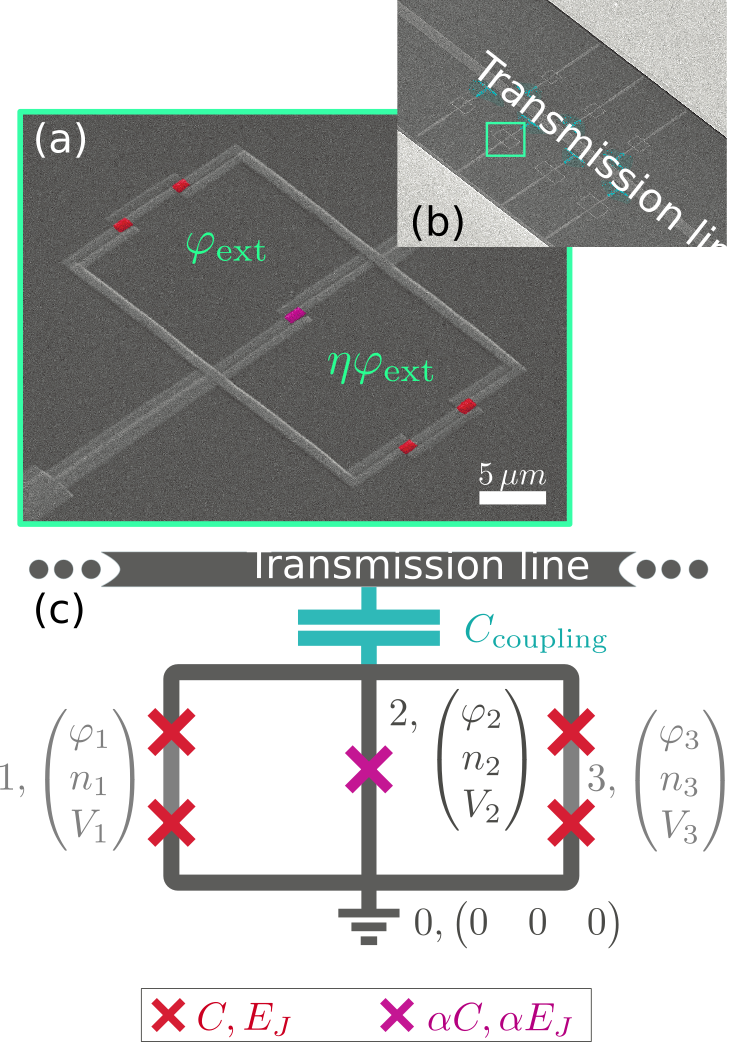
\includegraphics[width=8.6cm]{fig1}
  \caption{\small  \textbf{Geometry  of a  twin  qubit:}  (a) Scanning  electron
    microscope image of the twin qubit. The Al-AlO$_x$-Al JJs are highlighted in
    red and  pink; (b) Each  of the qubits is  coupled to the  transmission line
    with a T-shaped  capacitor; (c) The twin qubit is  a symmetrical arrangement
    of two individual  flux qubits \cite{Orlando_1999} sharing
    the central  JJ.  Islands are labeled  with a Cooper pair  occupation $n_i$,
    phase $\varphi_i$, with the  ground setting a reference of 0 for
    the variables.   JJs  (marked with  crosses)  mediate capacitive  and
    Josephson  interactions between  the islands.
  }
  \label{fig:setup}
\end{figure}

%% Describe fabrication
The sample is fabricated on an undoped silicon substrate, which is
pre-patterned with 100~nm Au ground planes. We  use electron beam lithography
and a shadow evaporation  technique to fabricate the qubit shown in
Fig.~\ref{fig:setup}(a). It consists of five JJs integrated into two
symmetrical  superconducting  loops. The  JJs  have  a   layered  structure  of
Al (20~nm) - AlO$_{\text{x}}$ - Al (30~nm).  The energy  and  capacitance of  the
central JJ  is a  factor of  $\alpha$ larger than  for the  outside ones,  which have
dimensions $400\times200$~nm$^2$.    The  coplanar  transmission   line  with
impedance $ Z_{0} \sim 50\,\Omega $ runs to the opening between the ground planes in the
center of the chip. The qubits are coupled to the transmission line
through T-shaped  capacitors.  An external magnetic field is applied to change magnetic flux bias in the identical loops.

%% Describe setup
The sample is mounted on a holder at the 13~mK
stage of  a dilution refrigerator.  A  superconducting shield is used  to screen
the holder  from stray magnetic  fields.  The RF  lines connected to  the sample
have attenuators for thermalization: -50~dBm on  the 50~K stage, -30~dBm on the
4~K  stage.  We  attach a  circulator on  the output  line for  isolation.  The
transmitted signal is amplified  by approximately +35~dBm on the 4~K stage  and by +35~dBm at
room  temperature.  This  set  of attenuators  and  amplifiers facilitate  power
conversion  between the  laboratory equipment  and the qubit.  Prior  to
charactering the qubit,  we  took  the microwave  transmission
spectrum with the qubit detuned, and  correct all measurements by subracting background
transmission profile.

Our primary goal  is to study the operation of the qubit in vicinity of a double degeneracy point $\Phi_0/2$, find the intrinsic energy structure and  compare with a numerical model of the system.

%% Measurement summary
We study the energy  spectrum  of the  twin qubit  by measuring transmission of coherent waves,  while  sweeping  the  biasing  magnetic flux.
The  \iket{1}~\ilra~\iket{2}  transition, is  mapped  with a  network
analyser which measures  the transmission of signal  $\omega_{\text{NA}}$ through the
system.
Away from  resonance the signal passes through the  circuit without any
interaction with the qubit so that the transmission
is close to  $ 100\% $.  Only near resonance  ($\omega_{\text{NA}}=\omega_{21}$), does the
qubit exchange photons  with the driving field as it  evolves between the ground
and excited states.  The  qubit emits a wave that is in anti-phase with
the driving  field \cite{Astafiev_2010}, so that the  destructive interference in
the output line results in  a transmission dip, see Fig.~\ref{fig:transmission}(a) inset. The plot shows power transmission $|t|^2$ obtained in a low limit drive and fitted by a Lorentzian curve with FWHM width $\Delta\omega/2\pi = 7$~MHz. This value gives us dephasing rate $\Gamma_2/2\pi \approx 3.5$~MHz.
%and we can derive the relaxation
%rate $\Gamma_1/2/pi \approx$~16~MHz according to $\Gamma_1/2\Gamma_2 = 1 - t_{min} $

Using the amplitude of the dip in the inset of Fig.~{\ref{fig:transmission}(a) we can estimate coupling of our qubit to the line\cite{Astafiev_2010,Peng_SPS}, which is characterised by the photon emission rate into the line $\Gamma_1^r =  2\Gamma_2 r_{0} \approx 0.6$~MHz, where $r_{0}$ is the reflection coefficient at the resonance.

The transmission minimum at different magnetic fields
maps   out   the   qubit's   $\omega_{21}$  transition   spectrum, Fig.~\ref{fig:transmission}(a).
Such a spectrum is observed in vicinity of external flux bias $\Phi \approx \Phi_0/2$ for all samples.
Because  of  a  small
asymmetry, $\eta\approx1$, the fluxes linked through  the left and right loops can be slightly
different: $ \Phi$ and $ \eta\Phi $, correspondingly. Eventually this results in gradual change of transmission frequency at large magnetic field, Fig~\ref{fig:transmission}(b).

\begin{figure}[h]
  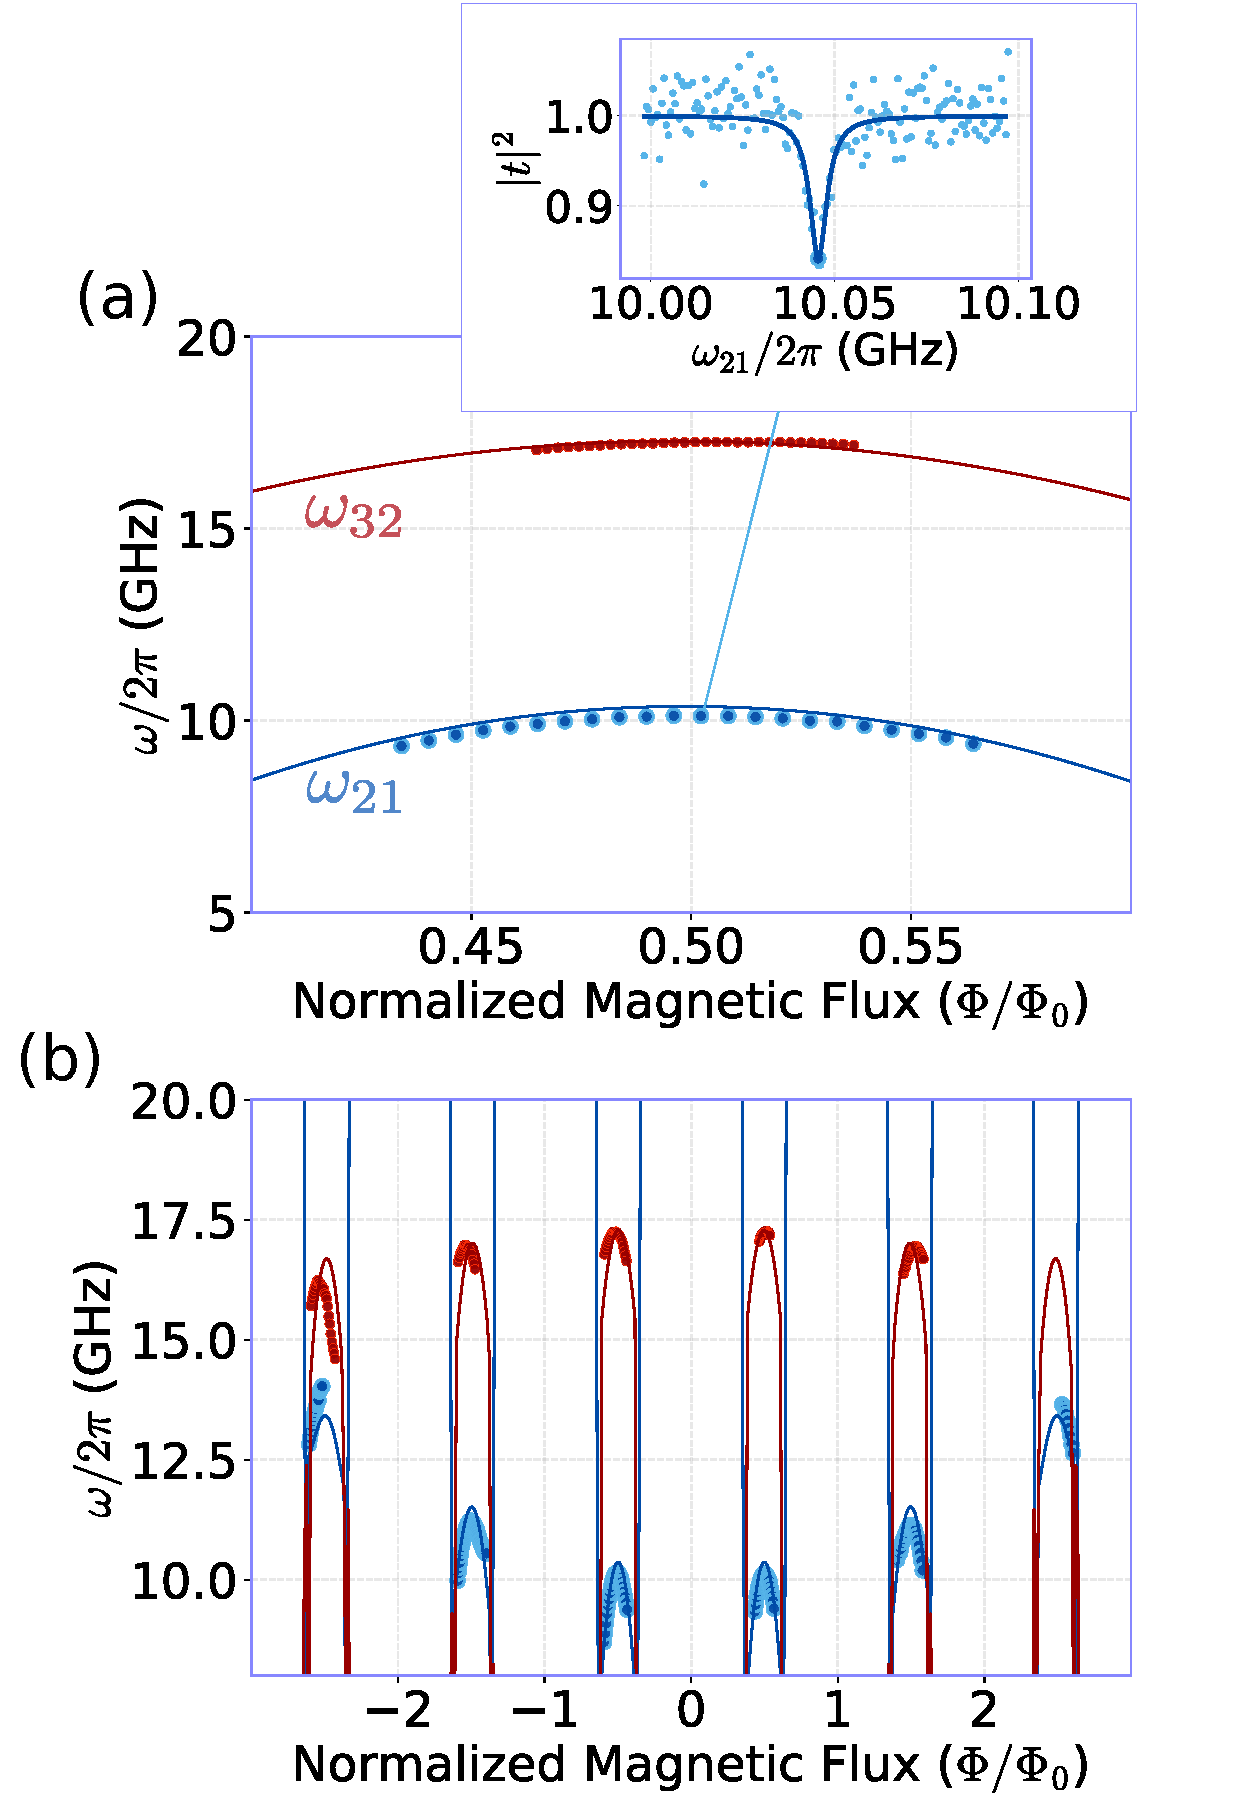
\includegraphics[width=86mm]{fig2}
  \caption{\small \textbf{Spectrum of the quantum system.} {\bf(a)}
    The resonance frequencies, $\omega_{21}$, in the vicinity of $\Phi_0/2$ (blue  points).
    An inset exemplifies the power transmission coefficient \,$\iabs{t}^{2} $\, for the \iket{1} \ilra \iket{2} transition.
    The transition frequencies
    $\omega_{32}$  (red) are obtained in a two-tone  measurement.
    {\bf{(b)}} The spectrum measured in a wide flux bias range. Experimental data (circles) are compared with
    simulations (solid lines) for $   \omega_{21}  $   (blue)  and
    $ \omega_{32}$ (red).  Asymmetry  in the flux penetrating the left and  right loops results in
    the  gradual   change  of   transition  frequencies   with  every   $  \Phi_{0}   $  period:
    $\omega_{21}$ creeps  up, while $\omega_{32}$ creeps  down, breaking the usual  periodicity of flux
    qubits.
    % Any changes to the probe's transmission are indicative of hitting the higher transition, which
    % is marked with a red point on the spectrum.
    % Readings are taken about the degeneracy point
    % $  \Phi \sim  \Phi_{0}/2 $,  where the  low  curvature of  transition energies,  allows for  stable
    % measurements with respect to fluctuations in the field.
  }
  \label{fig:transmission}
\end{figure}

The  \iket{2}\ilra\iket{3}  transition,  $\omega_{32}$,   is  mapped  using
spectroscopy with two tones. The network  analyzer probes  signals at  $ \omega_{21}  $, while  an
additional generator  sweeps a second  frequency, $ \omega_{\text{GEN}}  $.  Whenever
the second tone from the generator hits the \iket{2}\ira\iket{3} transition
($\omega_{\text{GEN}}  = \omega_{32}  $), the  qubit  undergoes a  ladder of  excitations,
\iket{1}  \iratext{$\omega_{21}$}\iket{2}  \iratext{$\omega_{32}$} \iket{3},  depopulating
states \iket{1} and \iket{2}.  Because of this depopulation, the probe signal at $\omega_{21}$ is
modified.
This identifies  $\omega_{32}$, which  is mapped  with red  circles, see Fig~\ref{fig:transmission}(b).
One can note that the qubit has a large anharmonicity in the two lowest transitions of more than 7.5~GHz.

We match the  experimental data to the theoretical model: Islands,  isolated by the
JJ  in  Fig.~\ref{fig:setup},  are  labeled with  Cooper  pair  (CP)  occupation
$       \vec{n}      =       \iket{n_1,      n_2,       n_3}      $,       phase
$     \vec{\varphi}     =     \iket{\varphi_1,     \varphi_2,     \varphi_3}     $  states.  The charges and potentials on
the islands are linked by the capacitance matrix:
\begin{equation}
  \label{eq:link}
  2e\vec{n} = \bold{C}\vec{V}.
\end{equation}
The capacitance matrix in the twin qubit topology is (see Supplementary Note I):
\begin{equation}
  \bold{C} = C \begin{pmatrix}
    2  &  -1  &  0\\
    -1  &  2  +  \alpha  &  -1\\
    0  &  -1  & 2
  \end{pmatrix},
  \label{eq:capac}
\end{equation}
where $C$  is the capacitance of the outer  JJs.  The interaction
of the  CPs, carrying a  charge $ \vec{Q}=2e\vec{n}  $, and potentials  on their
respective islands gives rise to the kinetic energy term (considering vortex motion) of the Hamiltonian:
\begin{equation}\label{eq:potential}
  \begin{aligned}
    T = E_C C \vec{n}^{T}\bold{C}^{-1}\vec{n},
  \end{aligned}
\end{equation}

\noindent where charging energy is $ E_{C}={(2e)^{2}}/{2 C } $.

Each  JJ  with  a  phase  difference  of  $\Delta\varphi_{i}$,  contributes $ E_{Ji}\big[1 - \cos(\Delta\varphi_i)\big] $ to a Josephson potential.   Additional phase due to external magnetic flux is accounted as an additional phase in left and right loops
$ \varphi_\text{ext} $ and $ \eta\varphi_\text{ext} $:
\begin{equation}\label{eq:kinetic}
  \begin{aligned}
    U  = &E_J\big[4 + \alpha - \alpha\cos(\varphi_{2}) -\cos(\varphi_{1}) -\cos(\varphi_{3}) - \\
    & \cos(\varphi_{2}   -  \varphi_{1}  -  \varphi_{\text{ext}})  -  \cos(\varphi_{2}   -  \varphi_{3}  +
    \eta\varphi_{\text{ext}})\big].
  \end{aligned}
\end{equation}
Here $\eta$ is a factor close but slightly different from one due to small asymmetry in the loop geometries.

The  Hamiltonian, $\mathcal{H}= T + U$, is  written  in  the charge  basis (see Supplementary Note II)  with
\iunit{E_J/h = 91.0}{GHz}, \iunit{E_C/h = 13.5}{GHz}, \iunit{\alpha = 1.023}{}, \iunit{\eta
  = 1.011}{}. The resulting eigenenergies are compared with the experimental data in
Fig.~\ref{fig:transmission}(b).  Data for $ \omega_{32} $ is taken in a limited flux range
because away from $ \Phi = (n + \frac{1}{2}) \Phi_0, n\in\mathbb{Z} $, the energy of $|1\rangle \leftrightarrow |2\rangle$ diverges below 0.4$\Phi_0$ and above 0.6$\Phi_0$.  The  asymmetry value, $ \eta $,  is close to
the  3\%  seen  from  the   SEM  image  in
Fig.~\ref{fig:setup}.  The  resonance is  periodic in flux,  with a  tendency of
higher $\omega_{21}$ at higher magnetic flux numbers, because of the loop asymmetry.

\begin{figure}
  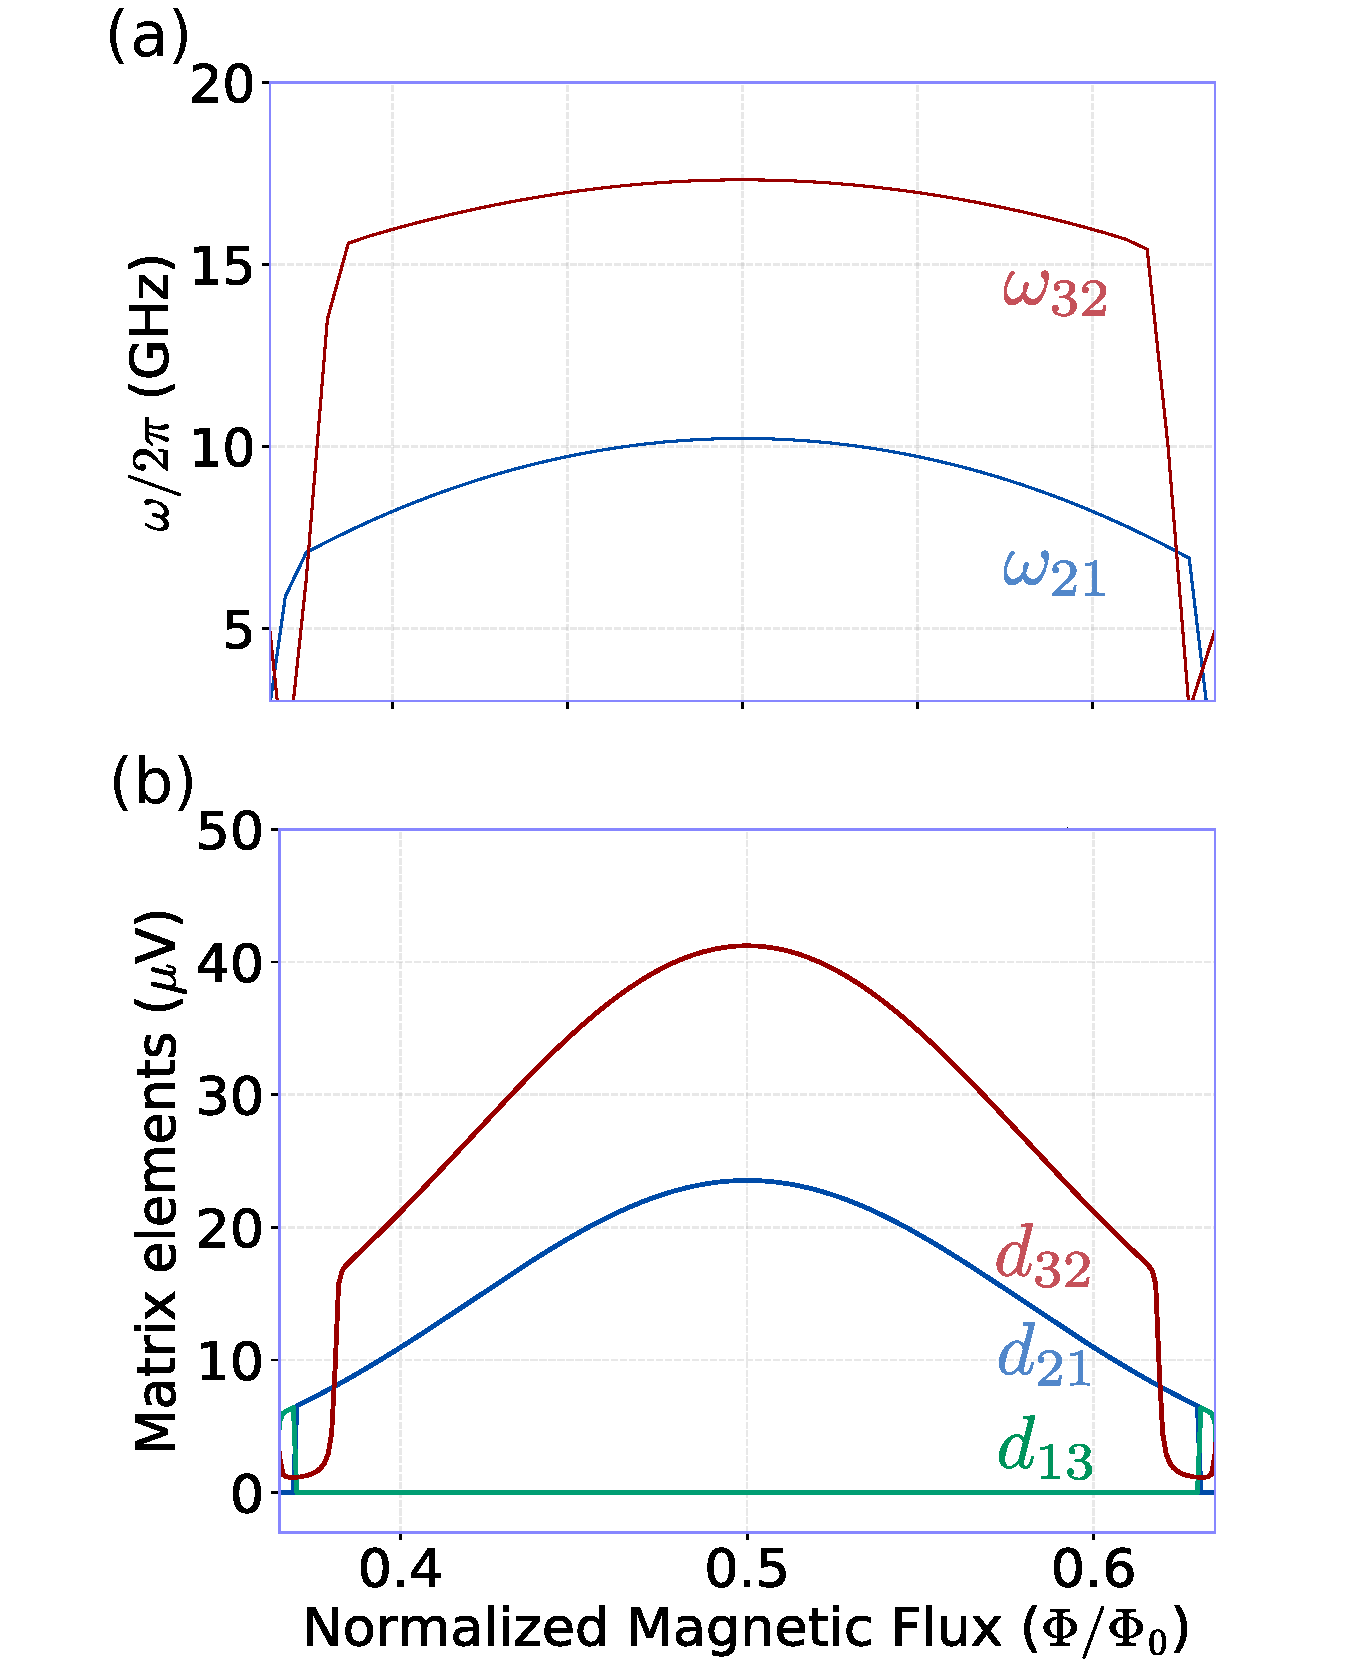
\includegraphics[width=86mm]{fig3}
  \caption{\small \textbf{Modelling the qubit.}
    (a) Calculations of transmission frequencies for the symmetric qubit,
    $\eta=1$. (b) Transition matrix elements $|d_{12}|$, $|d_{13}|$ and $|d_{12}|$ for the central island (Fig~\ref{fig:setup}).
  \label{fig:simulations}}
\end{figure}

An  important  parameter of the twin qubit is  the curvature at  the operation  point  of the  qubit, \,$\Phi_{0}/2$.  A  low curvature  is
desirable, because it  makes the  qubit less  sensitive to  external flux  changes and
improves  decoherence  time.   At   the  twin  qubits'  degeneracy  points
$      \Phi     =      (n+\frac{1}{2})\Phi_0,     n\in\mathbb{Z}      $,     the      curvature     is
$   (-550\pm10)\,\text{GHz}/\Phi_0^2  $.    It is substantially smaller than for 3-JJ and 4-JJ flux qubits with
similar JJ parameters \cite{Astafiev_2010, Stern_2014, Gustavsson_2012}, where the curvature is of the order of
$ 10^5$ $  \text{GHz}/\Phi_0^2$.

Figure~\ref{fig:simulations} shows simulation results for an ideal case of fully symmetric system ($\eta=1$). The curves are exactly periodic in magnetic filed with period of $\Phi_0$, therefore only one period is shown. The operational range of the qubit lies approximately from 0.43 to 0.57 of $\Phi_0$, where $\alpha$-junction is in the superposed 0-$\pi$ state\cite{Shulga_2018}. Away from that range the transition frequency $\omega_{21}$ diverges.


In addition, we analyse `optical' properties of our qubit.
Particularly, matrix elements $d_{12} = \ibra{1}\hat{V}_2\iket{2}$, $d_{13} = \ibra{1}\hat{V}_2\iket{3}$ and $d_{12} = \ibra{2}\hat{V}_2\iket{3}$ with physical meaning of induced potential on the island 2 due to atomic transitions between levels 1-2, 1-3 and 2-3 are calculated and plotted in Fig.~\ref{fig:simulations}(b). Here $\hat{V}_2 = (2e)^{-1}\partial H/\partial n_2$ is the potential operator for the island 2. It characterises coupling of the qubit to the field of propagating waves in the line, as well as its quantum fluctuations, responsible for photon emission. The calculation of the operator is given Supplementary notes.
%\begin{equation}
%  \label{eq:dv2}
%  \frac{E_{C}}{2\iabs{e}(1+\alpha)}\left[\hat{n}_1     +     2\hat{n}_2     +
%    \hat{n}_3\right].
%\end{equation}
It is interesting that $d_{13} = 0$\, for a wide magnetic flux interval, oppositely to a flux qubit where it happens strictly at the degeneracy point $\Phi_0/2$ only. This is due to symmetry of the system (two loops) to the external flux.

We estimate the photon emission rate using relationship\cite{Astafiev_2010,Peng_SPS} $\Gamma_1^r = (d_{12} C_k)^2 \omega Z_0/\hbar$ and found that the previously estimated value ($\Gamma_1^r/2\pi$ = 0.6~MHz) can be obtained if we substitute coupling capacitance $C_c =$~6~fF, which is very reasonable value for our geometry.

Finally, we measure Rabi oscillations, see Fig.~\ref{fig:rabi} by applying short microwave pulses with varied length. The oscillations decay with characteristic time $\tau_{\text{dec}}$~=~42~ns (Fig.~\ref{fig:rabi}),
It is consistent with the decoherence time taken from the spectroscopy measurements $\Gamma_2\approx1/\tau_{\text{dec}} \approx$~2$\pi\times$~3.8~MHz.
A relatively short decoherence time in our experiment is not surprising and can be a result of poisoning of  the sample
with  the infrared  radiation, and  the  coupling of the qubit to the two-level  oscillators in  the
substrate, owing to the simplified technology used in the qubit's fabrication. Note also that coherent operation is additionally limited due to strong coupling to the open line.

\begin{figure}
  \includegraphics[width=8cm]{fig5}
  \caption{\textbf{Rabi oscillations:}  taken at  the degeneracy point  by driving  the qubit
    with resonant microwaves pulses for fixed time periods, $ \Delta t $.  The decoherence time of
    $   \tau_{\text{dec}}  =   \iunit{42}{ns}  $   is   extracted  from   the  decay   envelope,
    $ e^{-\Delta t/\tau_{\text{dec}}} $, of the the oscillations. \label{fig:rabi}}
\end{figure}

In conclusion, we  have fabricated and  characterised an isolated  twin qubit.  With this geometry the qubit  has weak
flux  sensitivity at the degeneracy  point and strong anharmonicity. The measured energy level structure is well reproduced by the numerical model.

\section*{Acknowledgement}
\noindent The work was supported by the grants EPSRC~EP/T004088/1, H2020-FETOPEN-2018 QUANTUM ELEAPS, RSF No. 16-12-00070 for
supporting the work.

\bibliography{dipole_ilya_paper}

\end{document}
